\subsection{Eksempel}
Gennemgangen af metoden er beskrevet i detalje for hver del, men det kan være svært at få overblikket over metoden.
Af denne grund gives her et eksempel, der tager en fra de rå data og hele vejen til det aggregerede resultat.
Eksemplet, der følges kan ses i \cref{fig:totalbanjo}.
%intro godt at give et eksempel
%gennemgang af hvert led
%resultatet er at man har regnet ud der soves derfra og dertil
\begin{figure}
	\begin{minipage}{\linewidth}
		\begin{subfigure}{0.5\linewidth}
			\centering
			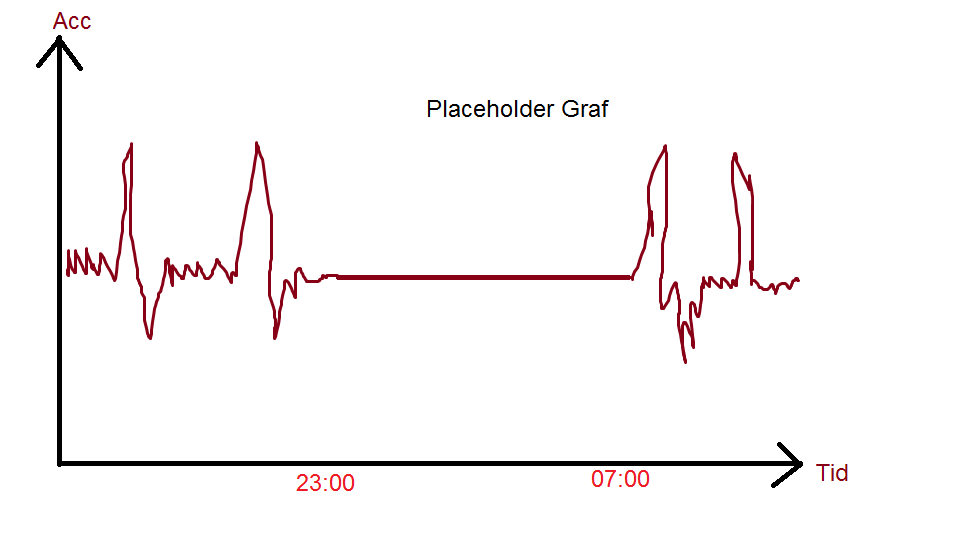
\includegraphics[scale=0.2]{acc-placeholder}
			\caption{Rå accelerations data.}\label{fig:rawaccplot}
		\end{subfigure}
		\begin{subfigure}{0.5\linewidth}
			\centering
			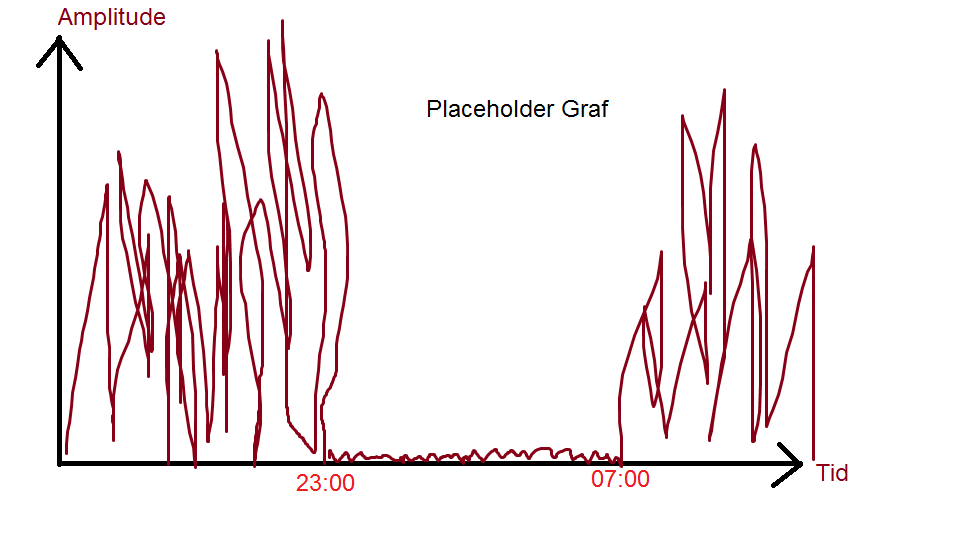
\includegraphics[scale=0.2]{ampl-placeholder}
			\caption{Rå amplitude data.}\label{fig:rawamplplot}
		\end{subfigure}
	\end{minipage}\\[1ex]%
	\begin{minipage}{\linewidth}
		\begin{subfigure}{0.5\linewidth}
			\centering
			
\includegraphics[scale=0.3, angle=270]{arrow}
		\end{subfigure}
		\begin{subfigure}{0.5\linewidth}
			\centering
			
\includegraphics[scale=0.3, angle=270]{arrow}
		\end{subfigure}
	\end{minipage}\\[1ex]%
	\begin{minipage}{\linewidth}
		\begin{subfigure}{0.5\linewidth}
			\centering
			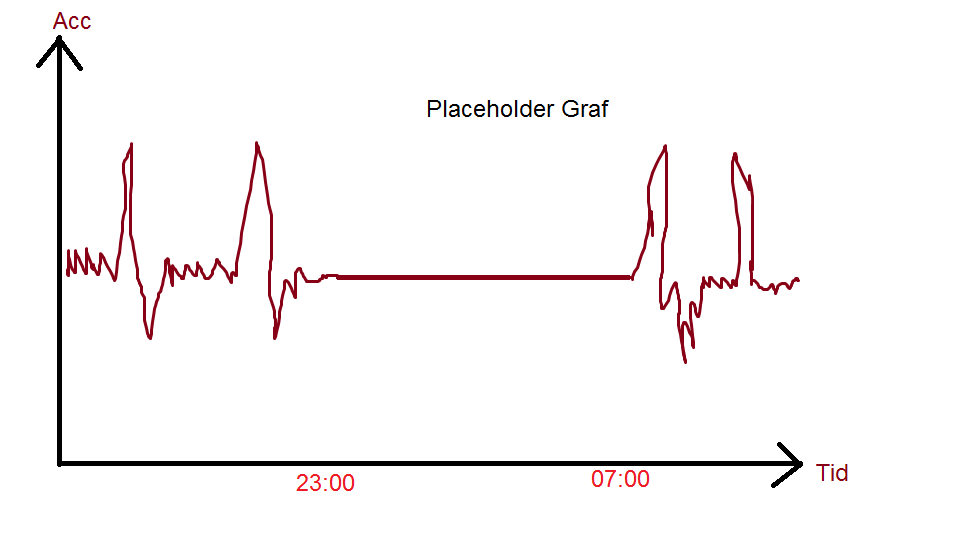
\includegraphics[scale=0.2]{acc-placeholder}
			\caption{Accelerations søvnestimering.}\label{fig:sleepcalcaccplot}
		\end{subfigure}
		\begin{subfigure}{0.5\linewidth}
			\centering
			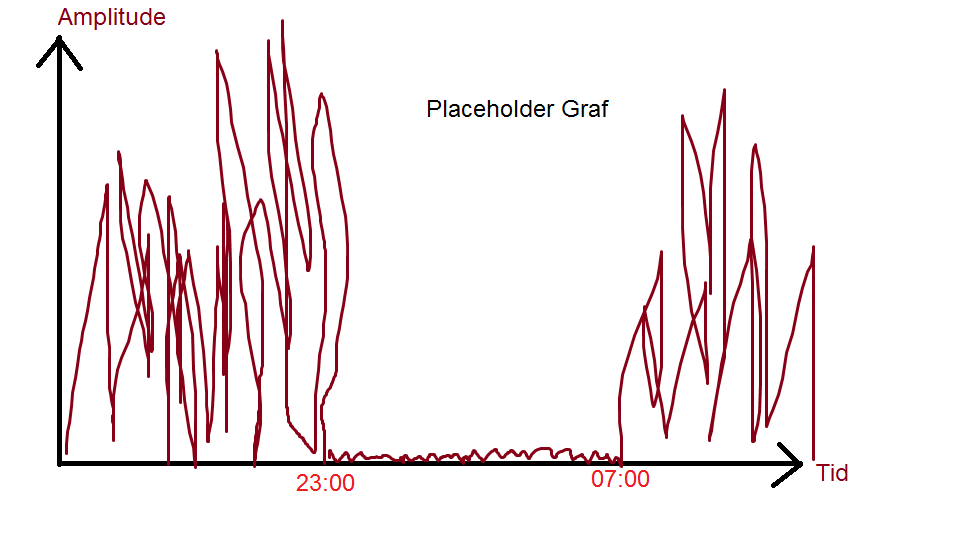
\includegraphics[scale=0.2]{ampl-placeholder}
			\caption{Amplitude søvnestimering}\label{fig:sleepcalcamplplot}
		\end{subfigure}
	\end{minipage}\\[1ex]%
	\begin{minipage}{\linewidth}
		\begin{subfigure}{0.5\linewidth}
			\centering
			
\includegraphics[scale=0.2]{downarrow}
		\end{subfigure}
		\begin{subfigure}{0.5\linewidth}
			\centering
			
\includegraphics[scale=0.2,angle=180]{uparrow}
		\end{subfigure}
	\end{minipage}\\[1ex]%
	\begin{minipage}{\linewidth}
		\begin{subfigure}{\linewidth}
			\centering
			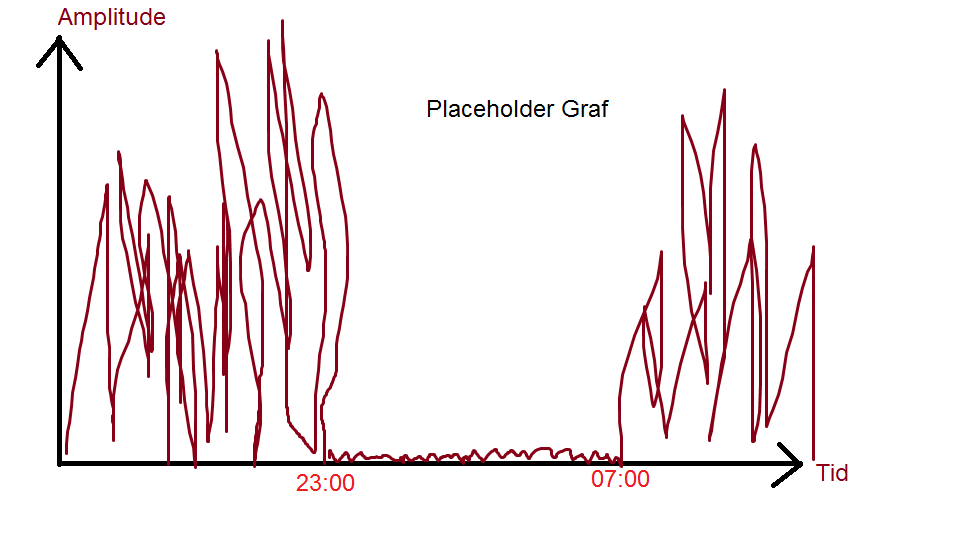
\includegraphics[scale=0.2]{ampl-placeholder}
			\caption{Kombineret søvnestimering}\label{fig:sleepcalcombine}
		\end{subfigure}
	\end{minipage}\\[1ex]%
	\begin{minipage}{\linewidth}
		\begin{subfigure}{\linewidth}
			\centering
			
\includegraphics[scale=0.3, angle=270]{arrow}
		\end{subfigure}
	\end{minipage}\\[1ex]%
	\begin{minipage}{\linewidth}
		\begin{subfigure}{\linewidth}
			\centering
			\begin{tabular}{|c|c|c|}
			\hline starttid & sluttid & sandsynlighed \\ 
			\hline 20-20-2015 00:01 & 20-20-2015 08:05 & 0.99 \\ 
			\hline 
			\end{tabular}
			\caption{Samlet søvnaggregeringsresultat.}\label{fig:finalagg}
		\end{subfigure}
	\end{minipage}
	\caption{Illustration af søvnestimering fra rå data til aggregering.}\label{fig:totalbanjo}
\end{figure}

Der startes med de rå accelerations og amplitude data, der kan ses i \cref{fig:rawaccplot} og \cref{fig:rawamplplot}.
På dette dataset foretages de beskrevne metoder, hvilket inkluderer et glidende gennemsnit, stilstandsbestemmelse og anvendelse af den logistiske funktion.
Vi kan allerede her observeret at der har været en stilstand omkring kl. 23 til kl. 7 næste dag.

Ud fra dette fås to separate søvnestimater, et fra accelerationsdata og et fra amplitudedata, og kan ses i \cref{fig:sleepcalcaccplot} og \cref{fig:sleepcalcamplplot}. 
Der kan observeres at søvnestimaterne følger stilstandsperioden fra omkring kl. 23 til kl. 7.

Disse estimater mangler dog at blive kombineret, og gøres ved brug af det beskrevne vægtede gennemsnit.
Som resultat deraf fås et estimat, som kan ses i \cref{fig:sleepcalcombine}.
Da dette estimat er et vægtet gennemsnit af de enkelte søvnestimater, kan man også her observere at det ser ud til at der er blevet sovet fra omkring kl. 23 til kl. 7.

Dette estimat er basis for aggregering, som skal foretages til at registrere hvorfra og hvortil man har sovet, der er det endelige resultat af estimeringen.
Dette resultat kan ses i \cref{fig:finalagg} og vurderer at ud fra det givne data er der sovet fra 23:26 til 07:00 næste dag.
\als{Ret til de tider vi ender ud med at bruge}